\chapter{Numbers 22}

\begin{figure}
  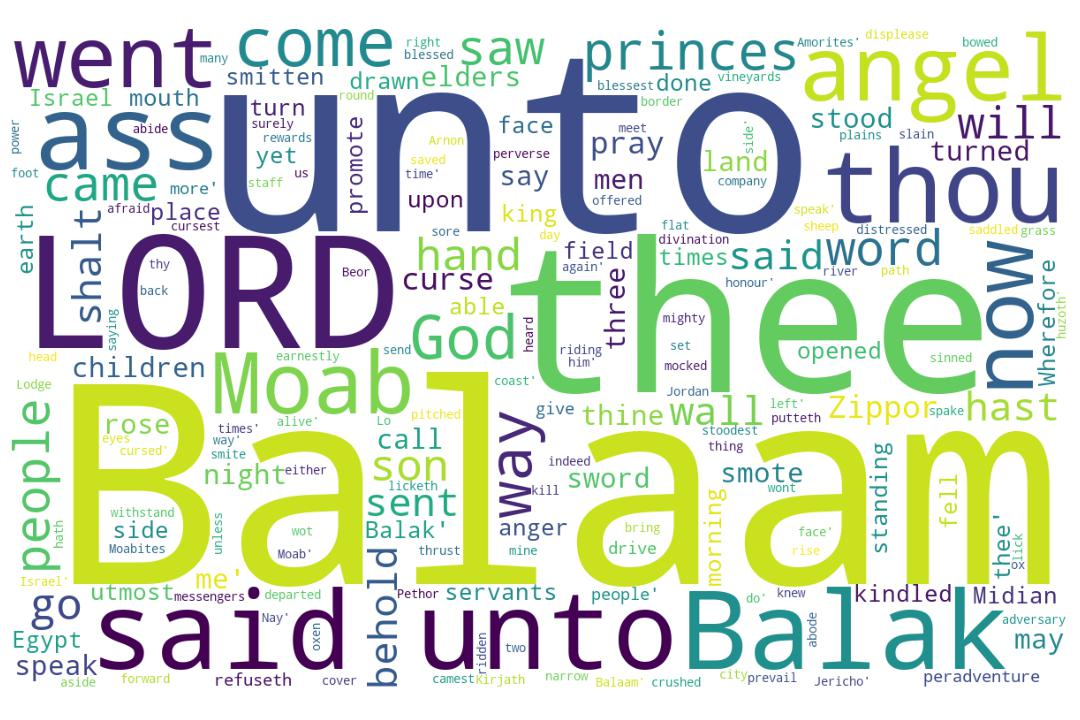
\includegraphics[width=\linewidth]{04OT-Numbers/Numbers22-WordCloud.jpg}
  \caption{Numbers 22 Word Cloud}
  \label{fig:Numbers 22 word Cloud}
\end{figure}

\marginpar{\scriptsize \centering \fcolorbox{bone}{lime}{\textbf{BALAAM'S RELIGION }}\\ (Numbers 22) \begin{compactenum}[I.][8]
    \item  \textbf{Assigned Diplomats} \index[scripture]{Numbers!Num 22:05}\index[scripture]{Numbers!Num 22:15} (Numbers 22:5, 15)
    \item  \textbf{Asking for Divination} \index[scripture]{Numbers!Num 22:07} (Numbers 22:7)
    \item Balaam's \textbf{Attempted Disobedience} \index[scripture]{Numbers!Num 22:19} (Numbers 22:19)
    \item \textbf{Armament Drawn} \index[scripture]{Numbers!Num 22:23}\index[scripture]{Numbers!Num 22:31} (Numbers 22:23, 31)
    \item The \textbf{Ass falls Down} \index[scripture]{Numbers!Num 22:27} (Numbers 22:27)
    \item An \textbf{Argument with a Donkey} \index[scripture]{Numbers!Num 22:29} (Numbers 22:29)
    \item An \textbf{Acquired Doctrine} \index[scripture]{Numbers!Num 23}\index[scripture]{Revelation!Rev 02:14} (Numbers 22, Revelation 2:14)
\end{compactenum}}

%%%%%%%%%%%%%%%%%%%%%%%%%%%%%%%%%%%%%
%%%%%%%%%%%%%%%%%%%%%%%%%%%%%%%%%%%%%
\footnote{\textcolor[rgb]{0.00,0.25,0.00}{\hyperlink{NumbersTOC}{Return to end of Table of Contents.}}}\footnote{\href{https://audiobible.com/bible/numbers_22.html}{\textcolor[cmyk]{0.99998,1,0,0}{Numbers 22 Audio}}}\textcolor[cmyk]{0.99998,1,0,0}{And the children of Israel set forward, and pitched in the plains of Moab on this side Jordan \emph{by} Jericho.}\\
\\
\P \textcolor[cmyk]{0.99998,1,0,0}{And Balak the son of Zippor saw all that Israel had done to the Amorites.}
[3] \textcolor[cmyk]{0.99998,1,0,0}{And Moab was sore afraid of the people, because they \emph{were} many: and Moab was distressed because of the children of Israel.}
[4] \textcolor[cmyk]{0.99998,1,0,0}{And Moab said unto the elders of Midian, Now shall this company lick up all \emph{that} \emph{are} round about us, as the ox licketh up the grass of the field. And Balak the son of Zippor \emph{was} king of the Moabites at that time.}
[5] \textcolor[cmyk]{0.99998,1,0,0}{He sent messengers therefore unto Balaam the son of Beor to Pethor, which \emph{is} by the river of the land of the children of his people, to call him, saying, Behold, there is a people come out from Egypt: behold, they cover the face of the earth, and they abide over against me:}
[6] \textcolor[cmyk]{0.99998,1,0,0}{Come now therefore, I pray thee, curse me this people; for they \emph{are} too mighty for me: peradventure I shall prevail, \emph{that} we may smite them, and \emph{that} I may drive them out of the land: for I wot that he whom thou blessest \emph{is} blessed, and he whom thou cursest is cursed.}
[7] \textcolor[cmyk]{0.99998,1,0,0}{And the elders of Moab and the elders of Midian departed with the rewards of divination in their hand; and they came unto Balaam, and spake unto him the words of Balak.}
[8] \textcolor[cmyk]{0.99998,1,0,0}{And he said unto them, Lodge here this night, and I will bring you word again, as the LORD shall speak unto me: and the princes of Moab abode with Balaam.}
[9] \textcolor[cmyk]{0.99998,1,0,0}{And God came unto Balaam, and said, What men \emph{are} these with thee?}
[10] \textcolor[cmyk]{0.99998,1,0,0}{And Balaam said unto God, Balak the son of Zippor, king of Moab, hath sent unto me, \emph{saying},}
[11] \textcolor[cmyk]{0.99998,1,0,0}{Behold, \emph{there} \emph{is} a people come out of Egypt, which covereth the face of the earth: come now, curse me them; peradventure I shall be able to overcome them, and drive them out.}
[12] \textcolor[cmyk]{0.99998,1,0,0}{And God said unto Balaam, Thou shalt not go with them; thou shalt not curse the people: for they \emph{are} blessed.}
[13] \textcolor[cmyk]{0.99998,1,0,0}{And Balaam rose up in the morning, and said unto the princes of Balak, Get you into your land: for the LORD refuseth to give me leave to go with you.}
[14] \textcolor[cmyk]{0.99998,1,0,0}{And the princes of Moab rose up, and they went unto Balak, and said, Balaam refuseth to come with us.}\\
\\
\P \textcolor[cmyk]{0.99998,1,0,0}{And Balak sent yet again princes, more, and more honourable than they.}
[16] \textcolor[cmyk]{0.99998,1,0,0}{And they came to Balaam, and said to him, Thus saith Balak the son of Zippor, Let nothing, I pray thee, hinder thee from coming unto me:}
[17] \textcolor[cmyk]{0.99998,1,0,0}{For I will promote thee unto very great honour, and I will do whatsoever thou sayest unto me: come therefore, I pray thee, curse me this people.}
[18] \textcolor[cmyk]{0.99998,1,0,0}{And Balaam answered and said unto the servants of Balak, If Balak would give me his house full of silver and gold, I cannot go beyond the word of the LORD my God, to do less or more.}
[19] \textcolor[cmyk]{0.99998,1,0,0}{Now therefore, I pray you, tarry ye also here this night, that I may know what the LORD will say unto me more.}
[20] \textcolor[cmyk]{0.99998,1,0,0}{And God came unto Balaam at night, and said unto him, If the men come to call thee, rise up, \emph{and} go with them; but yet the word which I shall say unto thee, that shalt thou do.}
[21] \textcolor[cmyk]{0.99998,1,0,0}{And Balaam rose up in the morning, and saddled his ass, and went with the princes of Moab.}\\
\\
\P  \textcolor[cmyk]{0.99998,1,0,0}{And God's anger was kindled because he went: and the angel of the LORD stood in the way for an adversary against him. Now he was riding upon his ass, and his two servants \emph{were} with him.}
[23] \textcolor[cmyk]{0.99998,1,0,0}{And the ass saw the angel of the LORD standing in the way, and his sword drawn in his hand: and the ass turned aside out of the way, and went into the field: and Balaam smote the ass, to turn her into the way.}
[24] \textcolor[cmyk]{0.99998,1,0,0}{But the angel of the LORD stood in a path of the vineyards, a wall \emph{being} on this side, and a wall on that side.}
[25] \textcolor[cmyk]{0.99998,1,0,0}{And when the ass saw the angel of the LORD, she thrust herself unto the wall, and crushed Balaam's foot against the wall: and he smote her again.}
[26] \textcolor[cmyk]{0.99998,1,0,0}{And the angel of the LORD went further, and stood in a narrow place, where \emph{was} no way to turn either to the right hand or to the left.}
[27] \textcolor[cmyk]{0.99998,1,0,0}{And when the ass saw the angel of the LORD, she fell down under Balaam: and Balaam's anger was kindled, and he smote the ass with a staff.}
[28] \textcolor[cmyk]{0.99998,1,0,0}{And the LORD opened the mouth of the ass, and she said unto Balaam, What have I done unto thee, that thou hast smitten me these three times?}
[29] \textcolor[cmyk]{0.99998,1,0,0}{And Balaam said unto the ass, Because thou hast mocked me: I would there were a sword in mine hand, for now would I kill thee.}
[30] \textcolor[cmyk]{0.99998,1,0,0}{And the ass said unto Balaam, \emph{Am} not I thine ass, upon which thou hast ridden ever since \emph{I} \emph{was} thine unto this day? was I ever wont to do so unto thee? And he said, Nay.}
[31] \textcolor[cmyk]{0.99998,1,0,0}{Then the LORD opened the eyes of Balaam, and he saw the angel of the LORD standing in the way, and his sword drawn in his hand: and he bowed down his head, and fell flat on his face.}
[32] \textcolor[cmyk]{0.99998,1,0,0}{And the angel of the LORD said unto him, Wherefore hast thou smitten thine ass these three times? behold, I went out to withstand thee, because \emph{thy} way is perverse before me:}
[33] \textcolor[cmyk]{0.99998,1,0,0}{And the ass saw me, and turned from me these three times: unless she had turned from me, surely now also I had slain thee, and saved her alive.}
[34] \textcolor[cmyk]{0.99998,1,0,0}{And Balaam said unto the angel of the LORD, I have sinned; for I knew not that thou stoodest in the way against me: now therefore, if it displease thee, I will get me back again.}
[35] \textcolor[cmyk]{0.99998,1,0,0}{And the angel of the LORD said unto Balaam, Go with the men: but only the word that I shall speak unto thee, that thou shalt speak. So Balaam went with the princes of Balak.}
[36] \textcolor[cmyk]{0.99998,1,0,0}{And when Balak heard that Balaam was come, he went out to meet him unto a city of Moab, which \emph{is} in the border of Arnon, which \emph{is} in the utmost coast.}
[37] \textcolor[cmyk]{0.99998,1,0,0}{And Balak said unto Balaam, Did I not earnestly send unto thee to call thee? wherefore camest thou not unto me? am I not able indeed to promote thee to honour?}
[38] \textcolor[cmyk]{0.99998,1,0,0}{And Balaam said unto Balak, Lo, I am come unto thee: have I now any power at all to say any thing? the word that God putteth in my mouth, that shall I speak.}
[39] \textcolor[cmyk]{0.99998,1,0,0}{And Balaam went with Balak, and they came unto Kirjath-huzoth.}
[40] \textcolor[cmyk]{0.99998,1,0,0}{And Balak offered oxen and sheep, and sent to Balaam, and to the princes that \emph{were} with him.}
[41] \textcolor[cmyk]{0.99998,1,0,0}{And it came to pass on the morrow, that Balak took Balaam, and brought him up into the high places of Baal, that thence he might see the utmost \emph{part} of the people.}